\section{Liste concatenate lineari}
Una lista concatenata lineare è una struttura composta da una collezione
di nodi collegati linearmente tra loro tramite puntatori.
Ogni {\textbf{nodo}} è contiene dei campi. Tra questi troviamo il campo {\emph{chiave}}, rispetto
al quale vengono effettuate le operazioni di ricerca, e il campo {\emph{pros}}, che contiene
un riferimento al nodo successivo. Nel caso delle liste ordinate, il campo {\emph{chiave}} 
viene utilizzato per determinare l'ordine tra i nodi. Si accede alla lista tramite un riferimento al primo nodo.
Le liste possono essere implementate tramite array o tramite strutture e puntatori. Noi studieremo il secondo
tipo di implementazione.
\begin{figure}[h]
    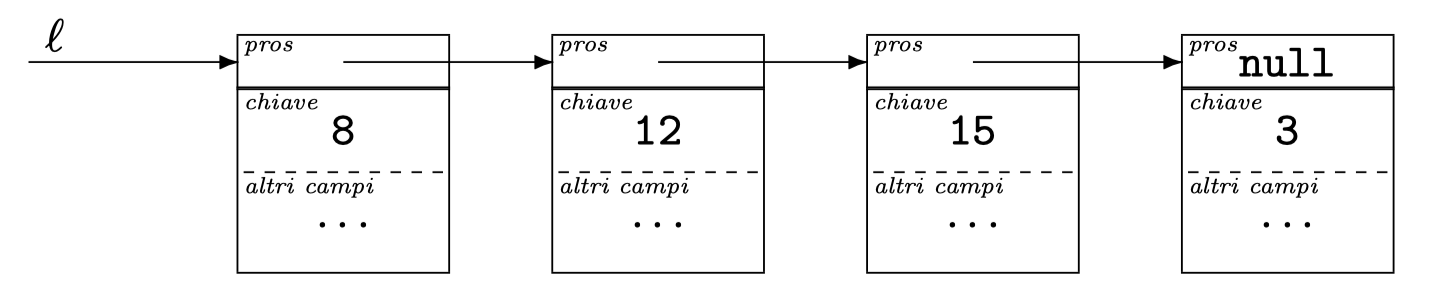
\includegraphics[width=\textwidth]{lista.png}
\end{figure}

\subsection{Operazioni}
Vediamo ora l'implementazione di alcune operazioni che si possono effettuare
sulle liste concatenate lineari ordinate e non.

\begin{figure}[h]
    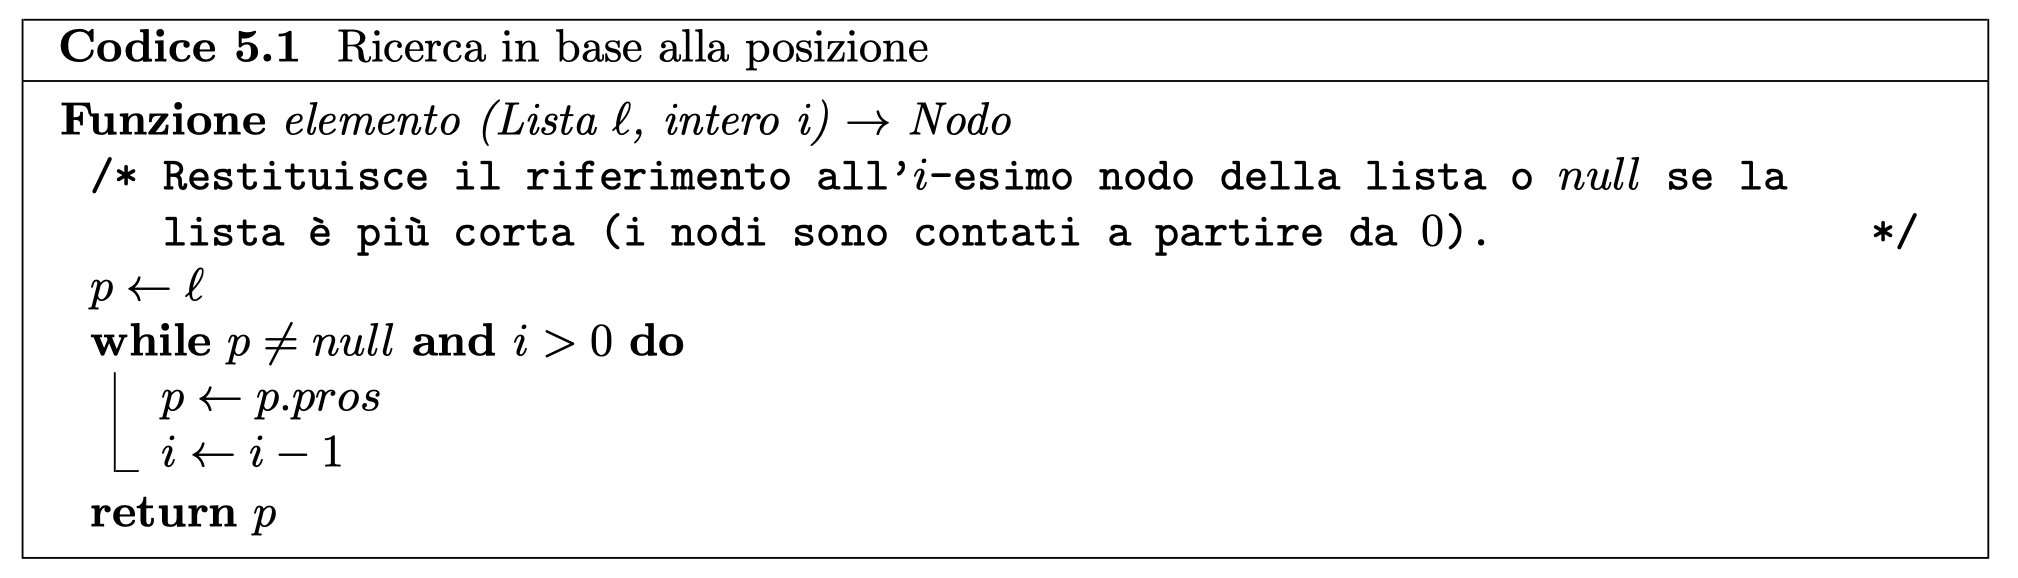
\includegraphics[width=\textwidth]{ricerca_posizione_lista.png}
\end{figure}

\begin{figure}[h]
    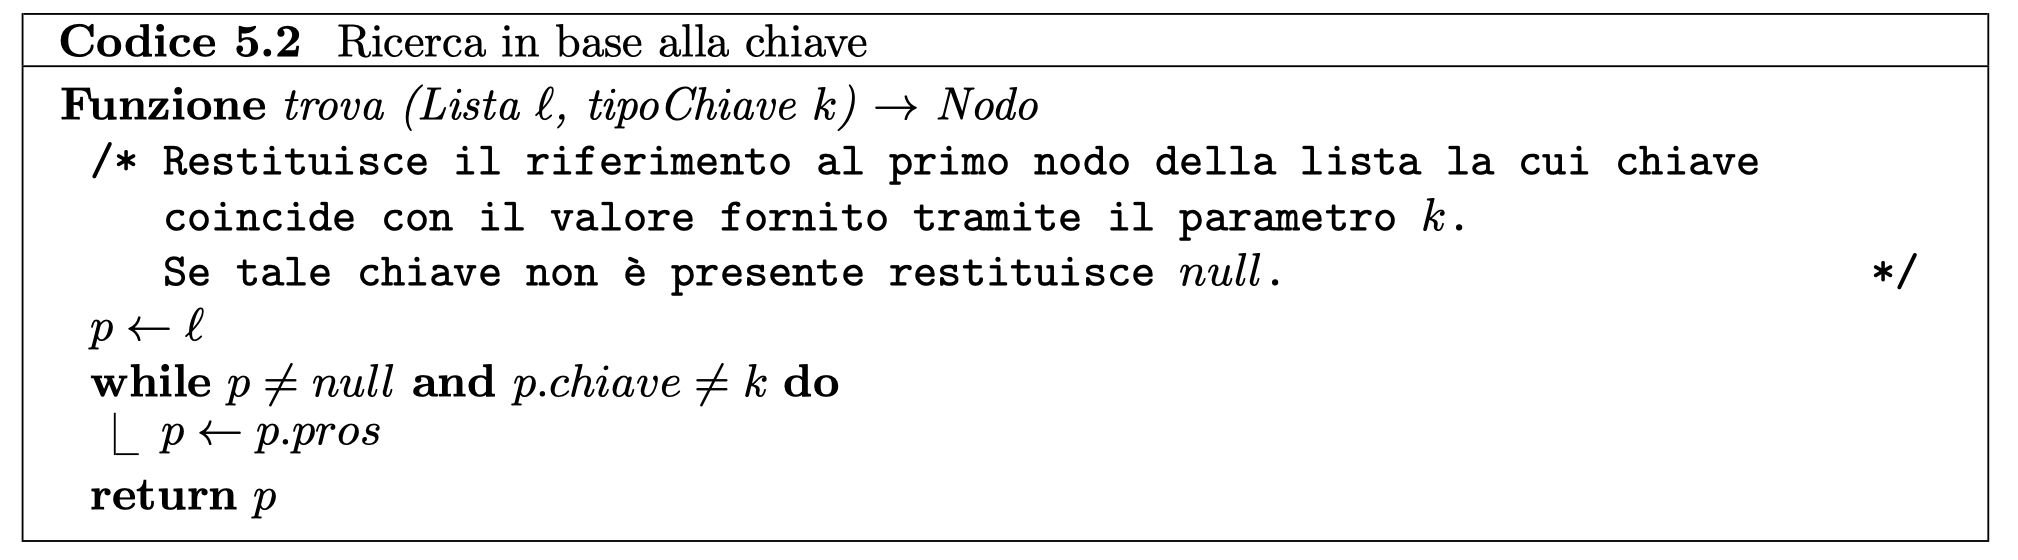
\includegraphics[width=\textwidth]{ricerca_chiave_lista.png}
\end{figure}

\begin{figure}[h]
    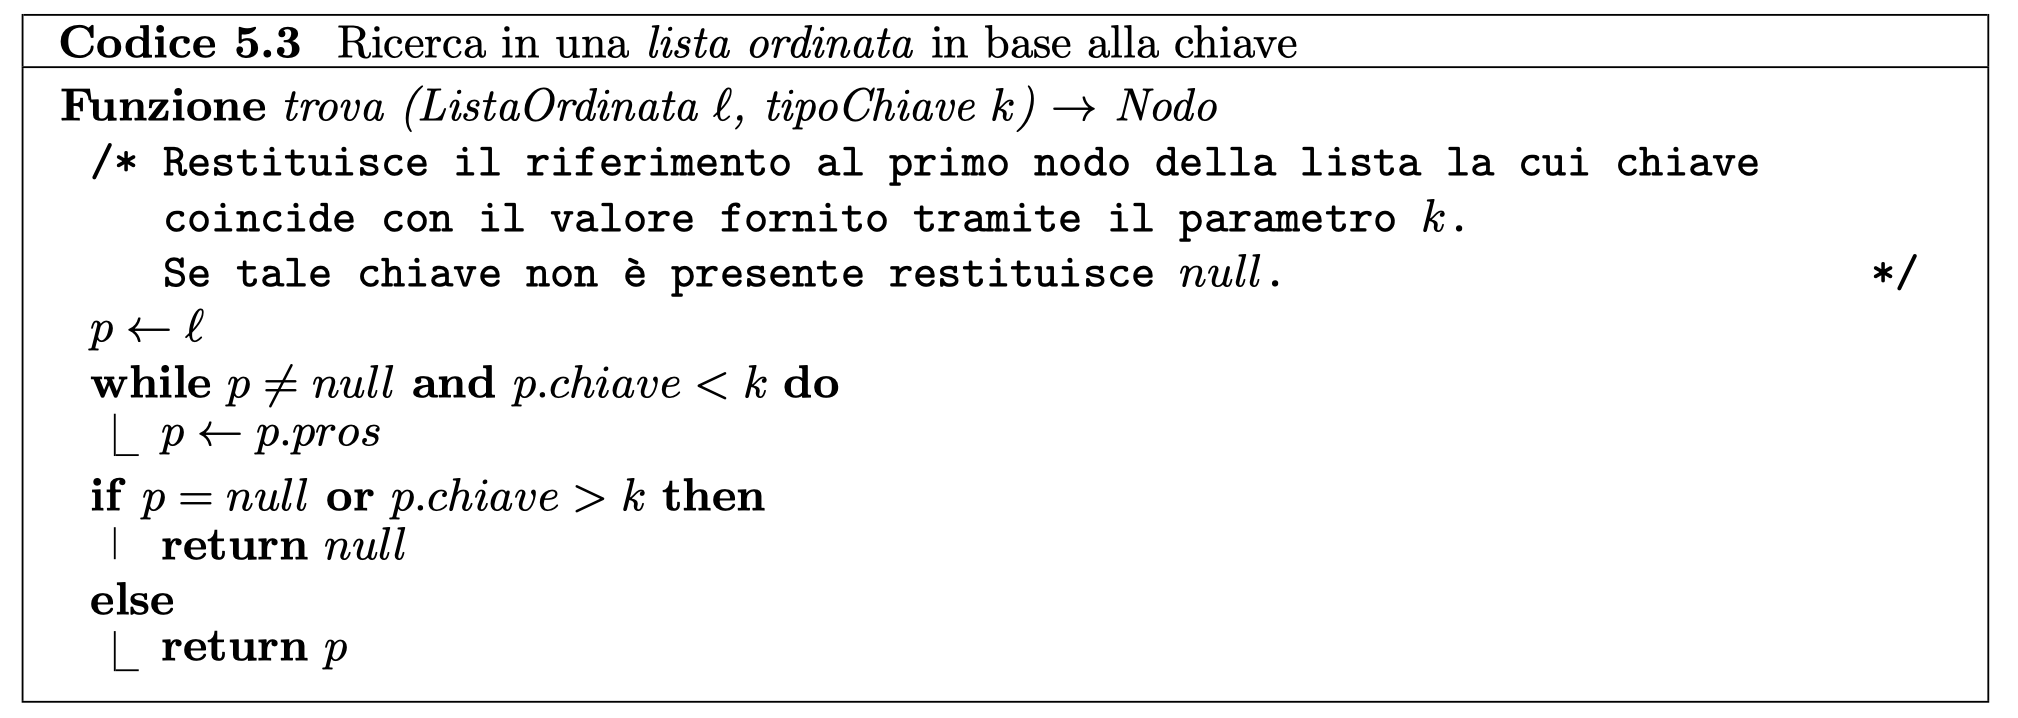
\includegraphics[width=\textwidth]{ricerca_chiave_lista_ordinata.png}
\end{figure}

\begin{figure}[h]
    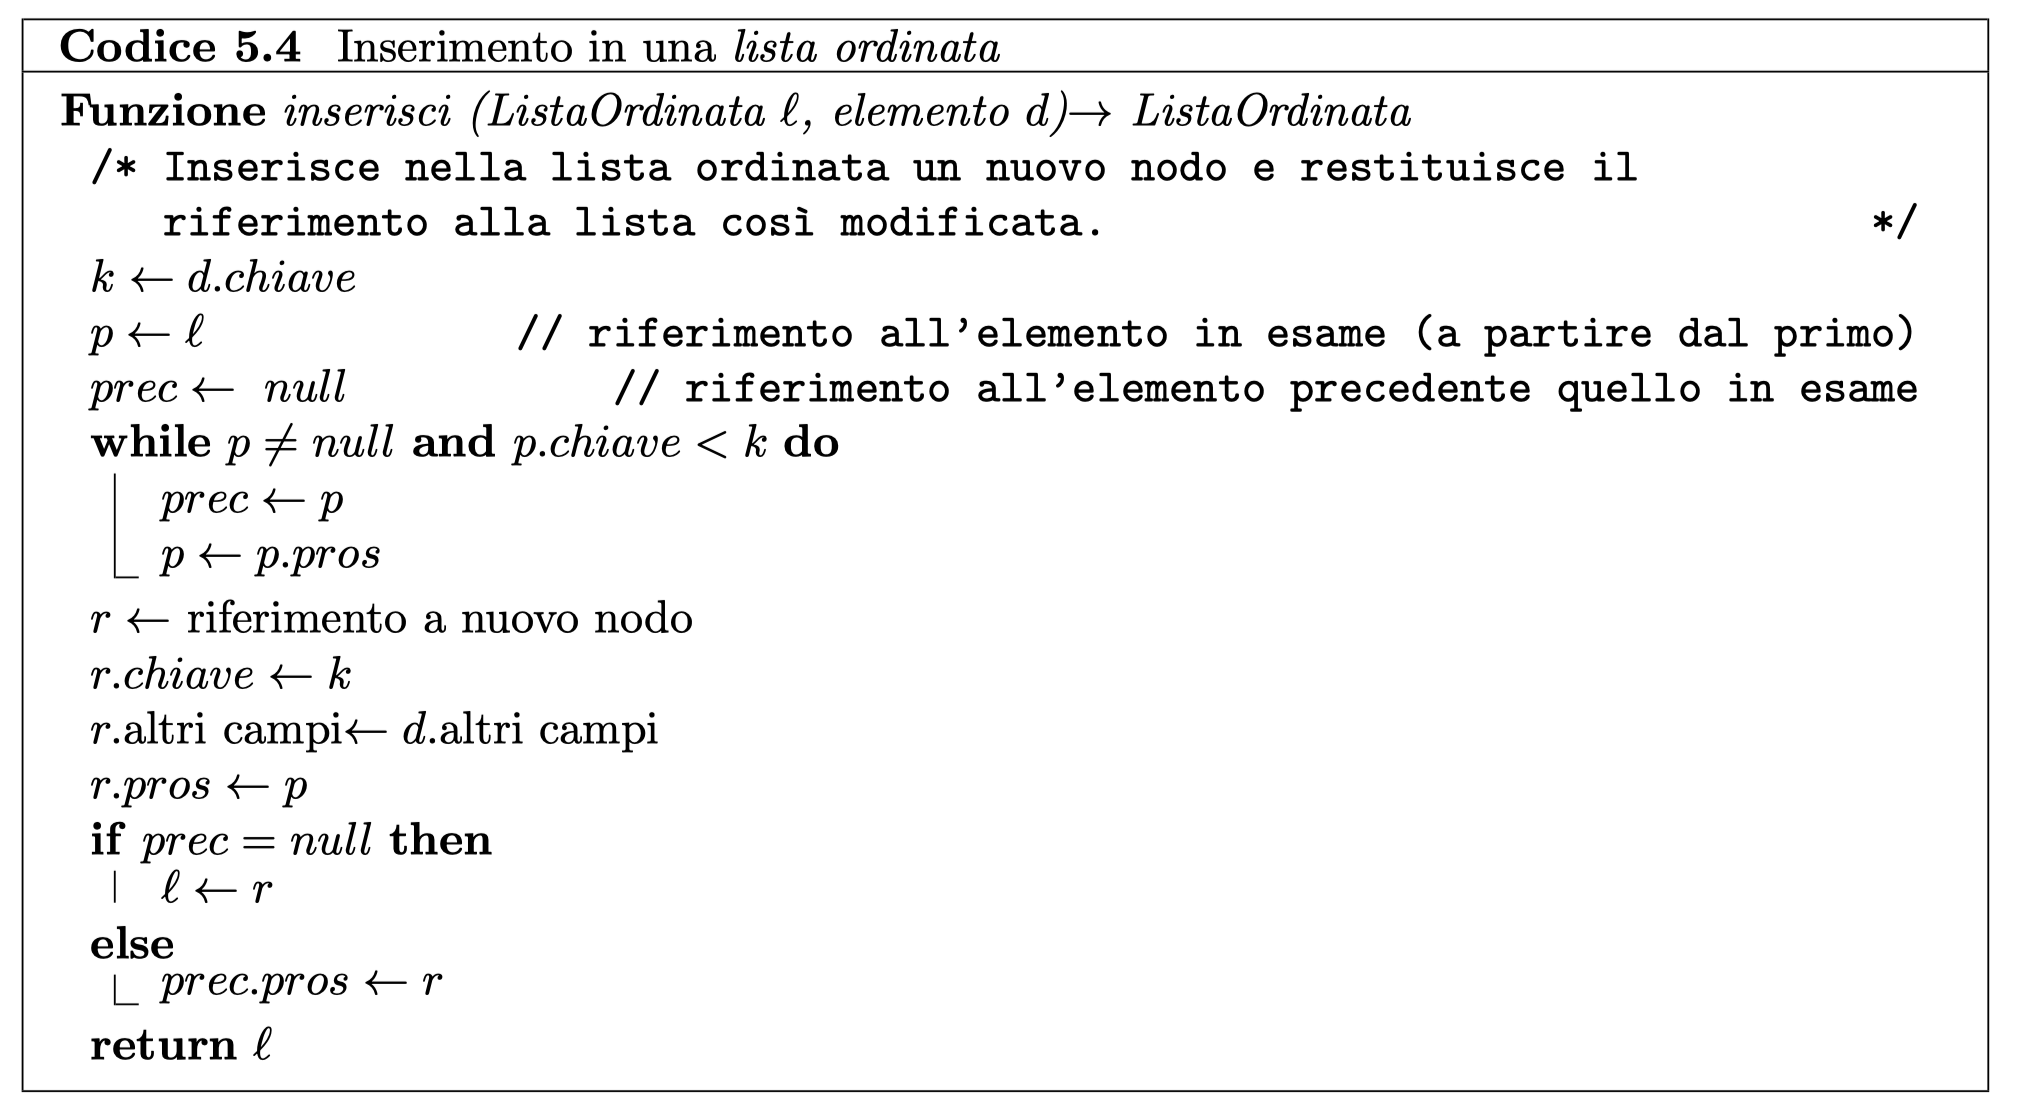
\includegraphics[width=\textwidth]{inserimento_lista_ordinata.png}
\end{figure}

\begin{figure}[h]
    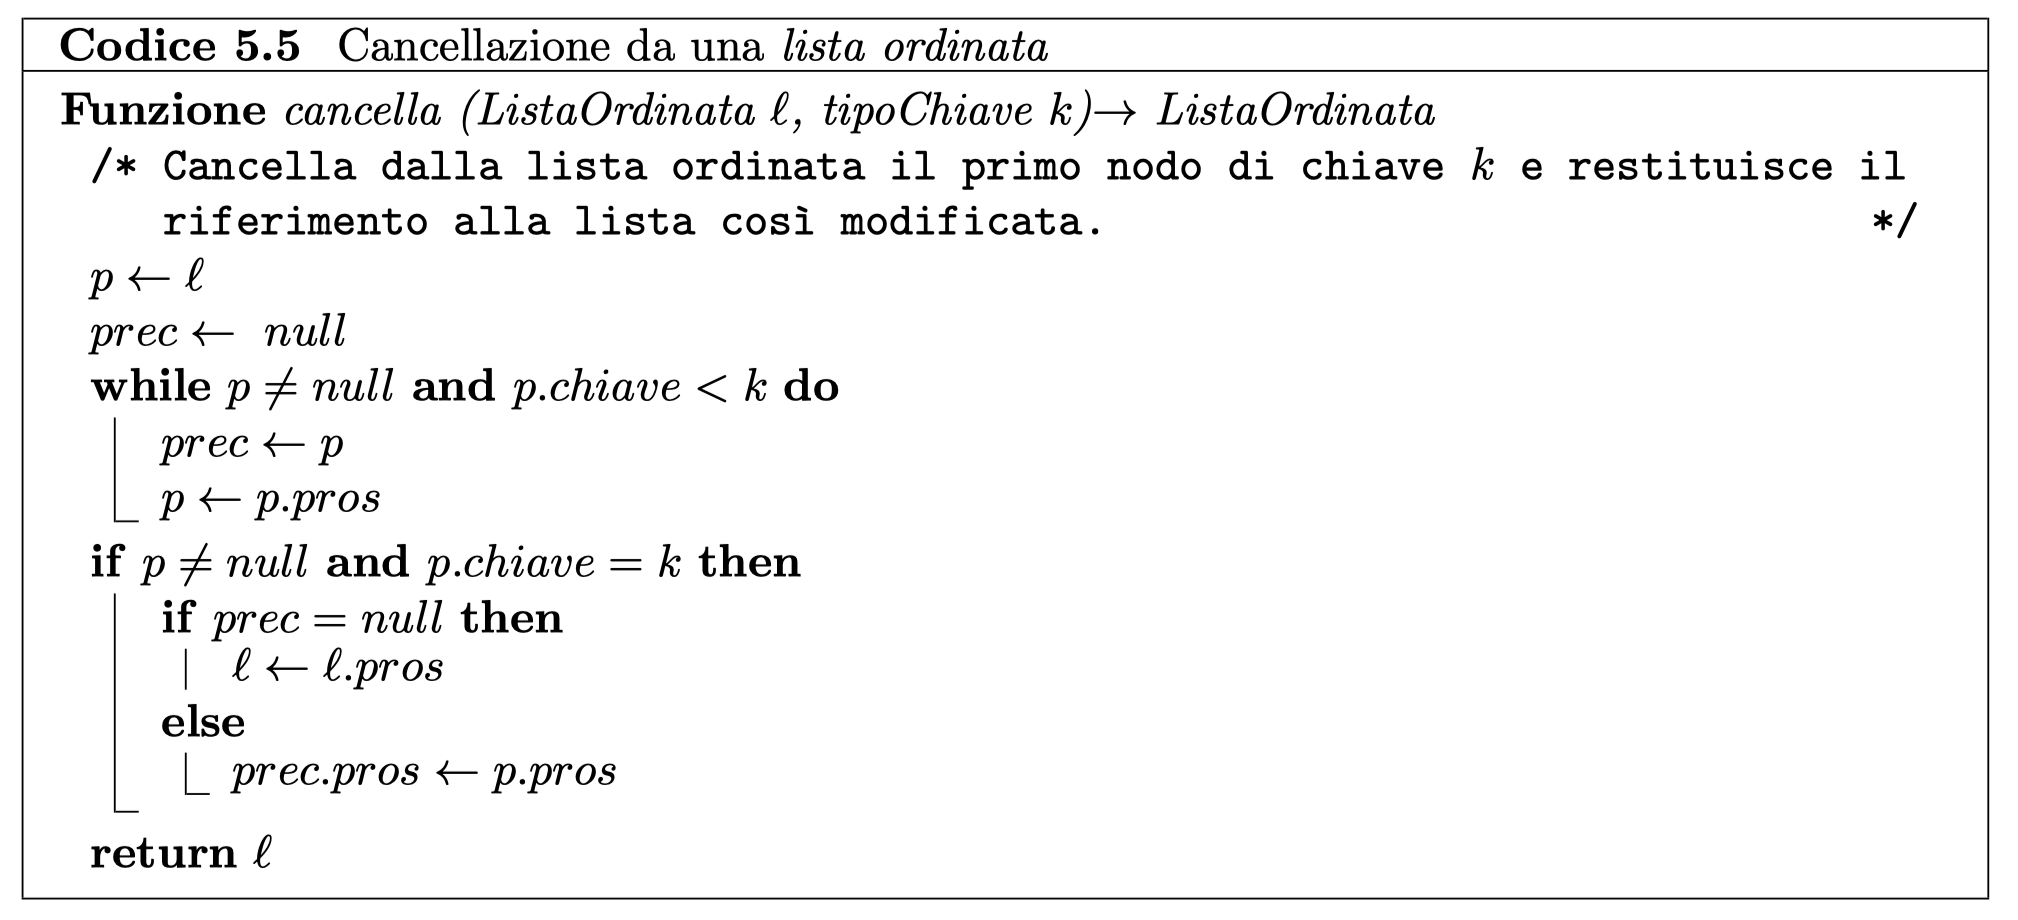
\includegraphics[width=\textwidth]{cancellazione_lista_ordinata.png}
\end{figure}
\clearpage